\section{System architecture and design}
The Energy Lens application aims to approximate the vision described in section~\ref{sec:vision}.  For our initial
attempt, we tagged items in a building with QR codes and allowed users to 1) tag and register new items, 
2) tell us which meters are attached to which items, and 3) scan individual item to view their load curve over a 
24-hour period.

The architecture consists of three layers: the sensing and tag layer, the data management and processing layer, and the application
layer.  In this section we discuss each layer and their most important components.  In deploying the application in a real building, 
we ran into various issues that informed our design.  For example, \emph{QR code reading times vary substantially across phones
and lighting conditions}.  You must design for the least-common demoninator in terms of camera quality and lighting.

Another aspect to consider is network access.  Within our building, although connectivity is mostly ubiquitous, network
access can be intermittent.  Network access may be unavailable for several reasons, including disassociation from an access point due
to idleness, dead spots in the building where connectivity to both wifi and 3G/4G are unavailable, multipath-induced
destructive interference, and various other reasons.  Dealing with these throughout the data collection and update phase is
especially troublesome.  We discuss various mechanisms and algorithms for dealing with disconnected operation.





\subsection{Sensing and tag layer}
We deployed 20 ACme power meters~\cite{acme} on a single floor of a building on campus.  The data was made available through
sMAP~\cite{smap} and forwarded to our processing and data management layer, StreamFS~\cite{streamfs}.  We distributed
the ACmes throughout a single floor in our building and registered various plug loads as being measured by them.  We also tagged
hundreds of items and locations throughout the entire building.  In total we tagged 20 meters, 20 metered items, 351 unmetered items,
 and 139 rooms.






\subsubsection{QR code design}
\label{sec:qrc}
Our choice to use QR codes is important, since the \emph{only way to scale -- in deployment size and management complexity -- is to
involve building occupants}. QR codes are cheap to produce.  They can be printed and attached to items with tape or sticky paper.  
Figure~\ref{fig:qrcexsecond} shows an example QR code used in our deployment.  These are placed on physical
objects and spaces throughout the building to link between the physical world and our virtual representation of it.

% With the number of physical objects and places in a building, \emph{we must rely on the occupants
% to scale our deployment and manage it over}. Because QR codes are easy to produce, we provide occupants with a webpage that
% that produces them.  They print them out, place them on items or places they want to interact with and register them.

Since occupants are our target users, we must make the application easy to use.  For QR code usage, varied lighting conditions, 
phone-specific camera quality, and shaky hand movements can make scanning cumbersome; ultimately de-motivating continued use.  
QR codes must be designed to minimize scanning time.  In our initial deployment and experiments we observe
that complex QR code code not only have an longer average scanning time but also experience a larger variance in scanning time.  
The more complex the pixel design in the QR code, the harder it is for the camera to focus and capture it. 


We scanned each QR code shown in Figure~\ref{fig:qrcexcomp}, under light and dark lighting conditions.  
Each experiment was run 10 times and Table~\ref{tab:qrscans} shows a statistical summary.  Scanning the simple QR code under well-lit 
conditions performed the best.  The complex QR code under  the same condition takes about 28-36\% longer to scan.
Perhaps even more important is the variance.  Notice that the variance with the simple QR code is smaller.
QR code image complexity increases with the amount of information you encode on it.  Therefore, it was imporant to decrease the
amount of information we encoded, \emph{placing the complexity in the lookup rather than the tag.}

\begin{figure}[htb!]
\begin{center}
\subfigure[Long QR Code.]{%
            \label{fig:qrcexfirst}
            
\includegraphics[scale=0.148]{figs/qrcexlong}
        }
\subfigure[Minimized QR Code.]{%
            \label{fig:qrcexsecond}
            
\includegraphics[scale=0.35]{figs/qrcex}
        }
\end{center}
\caption{
	The QR code on the left resolves to the same {\tt URL} at the right one, after resolution and
	redirection is complete. 
	The short label resolves to {\tt http://tinyurl.com/6235eyw}.  The second encodes about half
	the characters as the first.
	We used tinyUrl to reduce the QR code image complexity and scan time.
     }%
\label{fig:qrcexcomp}
\end{figure}

\begin{table}
\label{tab:qrscans}
\begin{center}
  \begin{tabular}{| r | c  c | }
    \hline
    			 & {\bf Average (sec) } & {\bf Variance (sec)} \\ \hline
    Short,light & 1.66 & 0.33 \\ \hline
    Short, dark & 2.08 & 0.35 \\ \hline
    Long, light & 2.26 & 0.71 \\ \hline
    Long, dark & 2.82 & 0.50 \\
    \hline
  \end{tabular}
\caption{Shows the time to scan a long QR code versus a short QR code in light and dark conditions (loosely defined).
Notice that short QR codes scan faster and with less variance that long ones.}
\end{center}

\end{table}

% Table~\ref{tab:qrscans} shows the results of some simple scanning experiment between the two tags
% shown above.  We scanned each QR code under light and dark lighting conditions, off the screen of my laptop.
% Each experiment was run 10 times and the table shows the statistical
% overview of the results. 
% Clearly, scanning the simple QR code under well-lit conditions
% performed the best.  The complex QR code under the same condition takes about 28-36\% longer to scan.
% On a generic QR code scanner, as used here, there is a portion of the
% scan time that is independent of the code complexity.  As these are
% more heavily used, this is expected to be reduced substantially and
% the difference is acquisition complexity will be even more pronounced.
% Perhaps even more important is the variance.  Notice that the variance with the simple QR code is much smaller and
% more stable under either condition.  In our experience, {\bf large variance in scan time is a major
% problem for complex QR codes}.  Thus we decided to re-design our codes and push more information in the lookup
% processes, as network access was more reliable than the focus of the camera on various mobile devices.
% Tags are placed on all types of devices in all kinds of locations with varying degrees of lighting.
% Simple QR codes are vital for widespread use.

% The design choice forced us to examine others that were related.  Not being able to encode much information on 
% our QR codes means we are more reliant on the network to provide the bulk of the information, to be very reliable,
% and to be widespread enough that disconnection is not problematic.  Moreover, there are a number of clients
% that can be used to access and display the information and the tag has to be meaningful for both.
% In order to meet these criteria we (1) shrunk {\tt URL}'s using tinyURL~\cite{tinyurl} as a level of 
% indirection and 
% (2) designed two classes of applications: \emph{shallow} applications, and \emph{deep-inspection} applications.  Shallow
% applications interact with the web-application directly while deep-inspection application use
% the {\tt URL} of the web application to extract a unique identifier and provide deeper inspection
% and update capabilities of the entity-relationship graph.

This is An example {\tt URL} we used in our deployment:{\tt http://tinyurl.com/6235eyw}.
When resolved, we get an empty response in the body, but we use the header to identify the QR code identifier 
that we associate with the item.  The response header looks as follows:

\begin{figure}[htb!]
\begin{center}
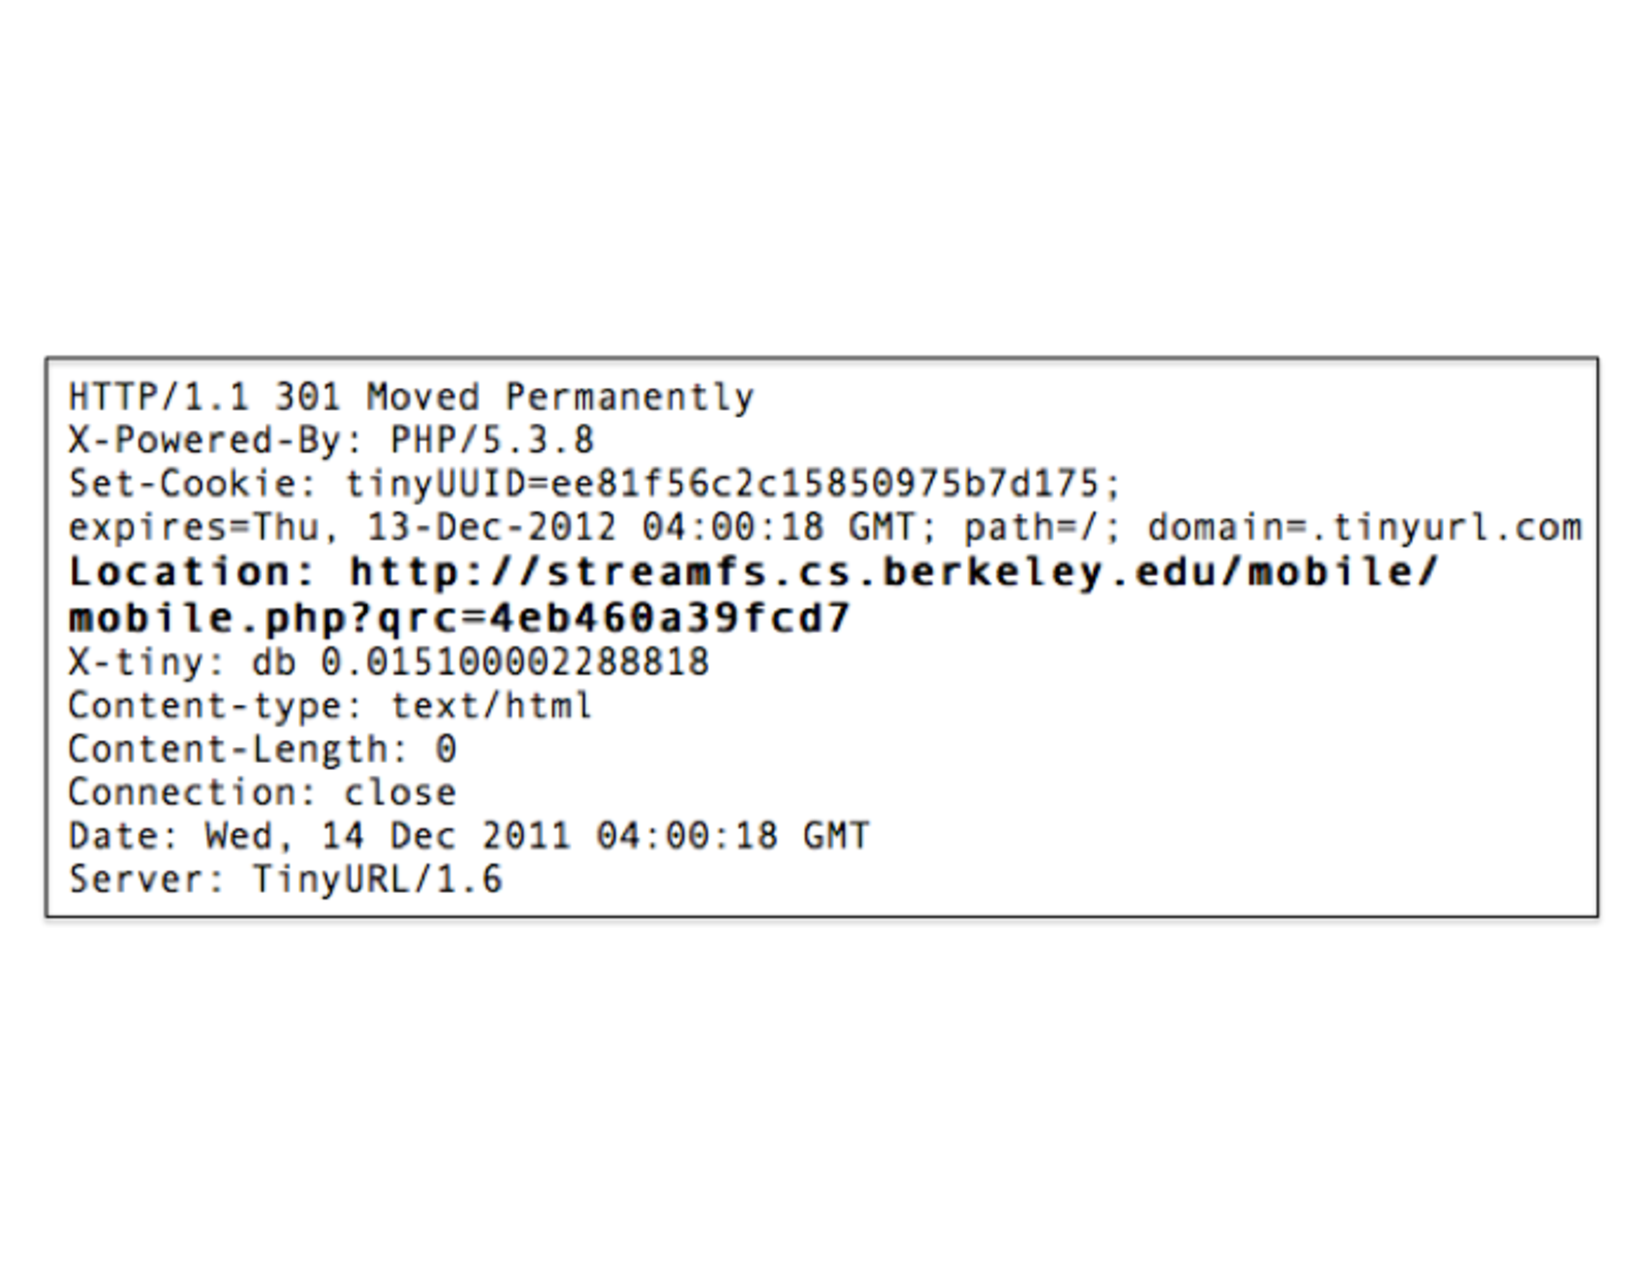
\includegraphics[scale=0.30]{figs/tinyurlhdr}
\caption{The header of the response from the {\tt tinyUrl} when resolving a QR code.  The `Location' attribute
is used to extract the unique identifier for the object this QR code tags.  It is also used to re-direct
users without the phone application to a meaningful web address for the object.}
\label{fig:tinyurlhdr}
\end{center}
\end{figure}


Notice the `Location' attribute in the header.  This is the location of the re-direct.  This approach gives us
flexibility in several ways:

\begin{enumerate}
\item It allows us to encode less information in the QR code, descreasing its visual construction, making it more
		robust across phones with different camera quality, poor lighting conditions, and shaky hands.
\item It allows the added layer of indirection to serve two versions of the applications:  the native application,
		where users can \emph{deeply explore} and edit the entities and their relationships and the \emph{shallow lookup}, 
		which re-directs the mobile phone to a read-only view of the item that was scanned -- such as a power trace or 
		a description.
\end{enumerate}


% It provides a web address for users to re-direct to and find information and various read-only services for the object.  However, because
% the {\tt URL} also contains a unqiue identifer \emph{qrc}, it can be used to provide for sophisticated services and capabilities.
% An example is the ability to change the virtual structure of inter-relationship between this object and other objects.  This
% is demonstrated in our energy auditing application discussed in detail in section~\ref{sec:eaudit}.
% Once items are tagged, they can be added and removed by swiping the tag and pressing the button for what you want to do with
% the item.  You also check into locations either explicit with a location-tag swipe or implicitly with an item swipe.

% \emph{Shallow} applications
% use the {\tt URL} directly.  The \emph{qrc} {\tt URL} is unqiue identifier for the item that this tag is attached to.
% A shallow application can obtain mostly read-only service through our web applications.  For example, we'll see how
% to get either item-specific data or item-aggregated data with respect to the user making the request (i.e. the total
% energy consumed by \emph{my} devices).  \emph{Deep-inspection} applications are native to the phone, so we can do much
% more with the tag.  Our energy auditing application allows you to related the item to other items by maintaining state of swipe
% history.  This is more difficult with the web-applicaiton.  We can also use the tag and item information to couple it with
% sensor information coming from sensors on the phone itself.  For example, we could determine the direction an object
% is pointing by using the phone's directional sensor and negating their direction (i.e. phone is facing east, tag on item must
% be facing west).

% \begin{figure*}[htb!]
% \begin{center}
% 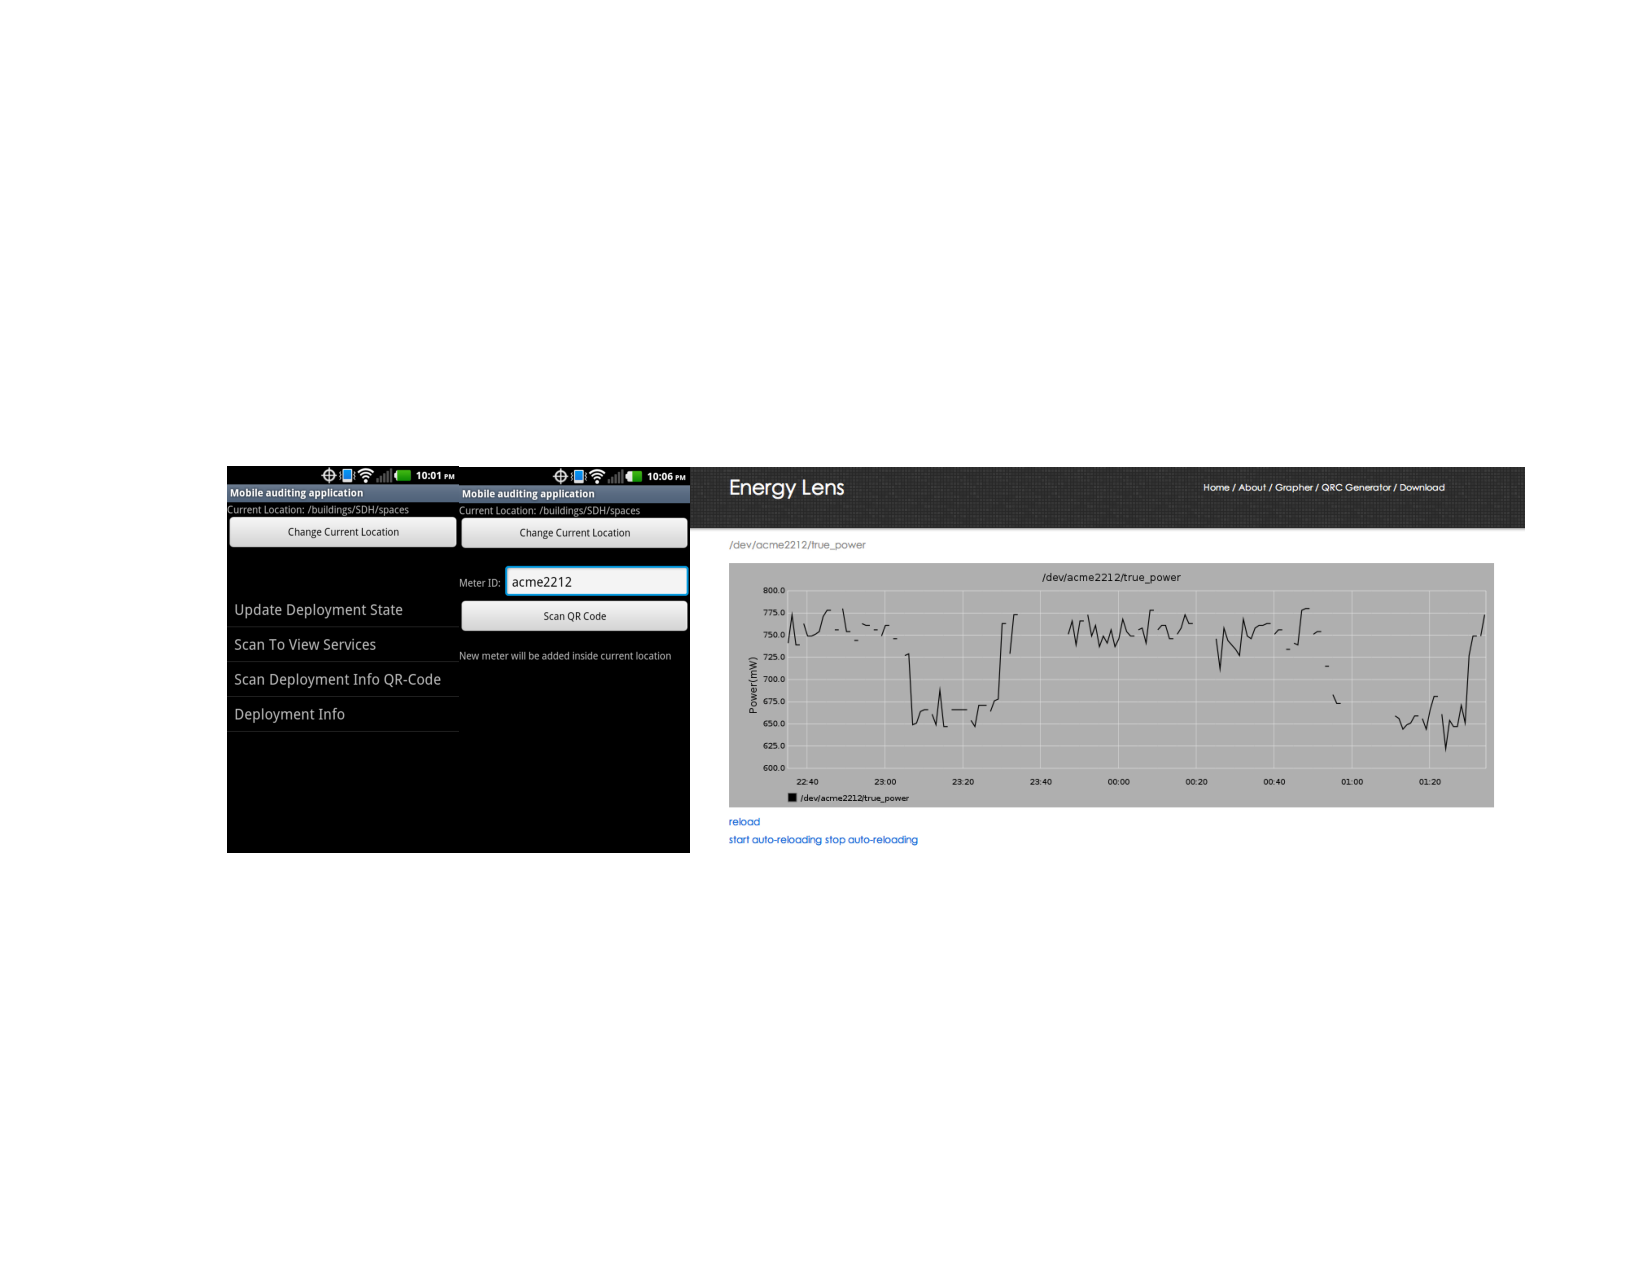
\includegraphics[width=\textwidth]{figs/mobileapp}
% \caption{Screen shots of the mobile application.  The screens on the left are for editing the state of the deployment.
% The graph on the right shows a live feed of a the sensor that's attached to the item that was scanned with the `Scan To
% View Services' option in the mobile application.  It can also be resolved by scanning the QR code and following the re-direct
% to the URL.}
% \label{fig:mobileapp}
% \end{center}
% \end{figure*}


\subsection{Data management layer}
ACme meters are IP-enabled and forward their data through a router that runs sMAP.  sMAP then forward the incoming data
to StreamFS, running in a machine in Amazon's EC2.  StreamFS is a web service that organizes streaming data and metadata using
a hierarchical naming convention.  It also provide a pub/sub facility for streaming data.  We construct 
a cononical naming convention within StreamFS to express the entity relationships between people, things, and meters.  The pub/sub
mechanism allows us to combine the ERG with streaming data, and feeds our timeseries data viewers.

\subsubsection{Entity-Relationship graph}
We construct the entity relationship graph through naming in StreamFS.  StreamFS uses filesystem constructs, such as symbolic
links and hiearchical naming which are useful for expressing an acyclic graph structure -- StreamFS disallows symlinks that causes cycles.  
The following general path naming patterns are use to experess different portions of the ERG.
% $/path/to/device\_or\_item$, 
% $/path/to/qrc$, $/path/to/space$, $/path/to/taxonomy$, $/path/to/users$.  
The first path is actually {\tt /dev}.  This directory
holds all registered meters.  Items are stored in {\tt /inventory}.  QR codes are stored in {\tt /qrc}.  When an item is registered an 
symbolic link is created from the specific qr code directory to the item.  {\tt /spaces} contains a hierarchy of floors, rooms, 
and sub-spaces.  The placement association is captured with symbolic links as well.

The various types inform the application of the nature of the relatinonship.  The types are item, meter, 
location, category, and tag.  The following relationships we capture are:

\begin{itemize}
\item {\bf Owned-by}: When a meter/item/location is tagged as belonging to a user.
\item {\bf Bound-to}: When a meter is attached to an item and taking physical measurements associated with that 
		device, we say that the meter is ``bound-to'' the device.
\item {\bf Attached-to}: When a meter/qr code/item is attached to another meter/qr code/item but NOT taking any 
		physical measurements for that item, we say that the meter/item is ``attached-to'' the other meter/qr 
		code/item.  QR codes should not be attached to each other and are not accepted by the EnergyLens application.
\item {\bf Is-in}: When a meter/item is inside a location, we say that the meter/item ``is-in'' that location.
\item {\bf Type-of}: When an item is labeled by as a known, specific, type, we say that the item is a ``type-of'' thing 
		specified by the its label.
\end{itemize}

All symlinks are interpretted based on these rules of association.  As items move, symlinks are removed and re-created
in a different folder.  We know your current location by following the path from the QR code directory, across a symlink, 
to a file in the space directory.  Items associated with a space have a floor or room folder point to the item
via a symlink.  This is how we record the location of things throughout the building.

% \begin{figure}[htb!]
% \begin{center}
% 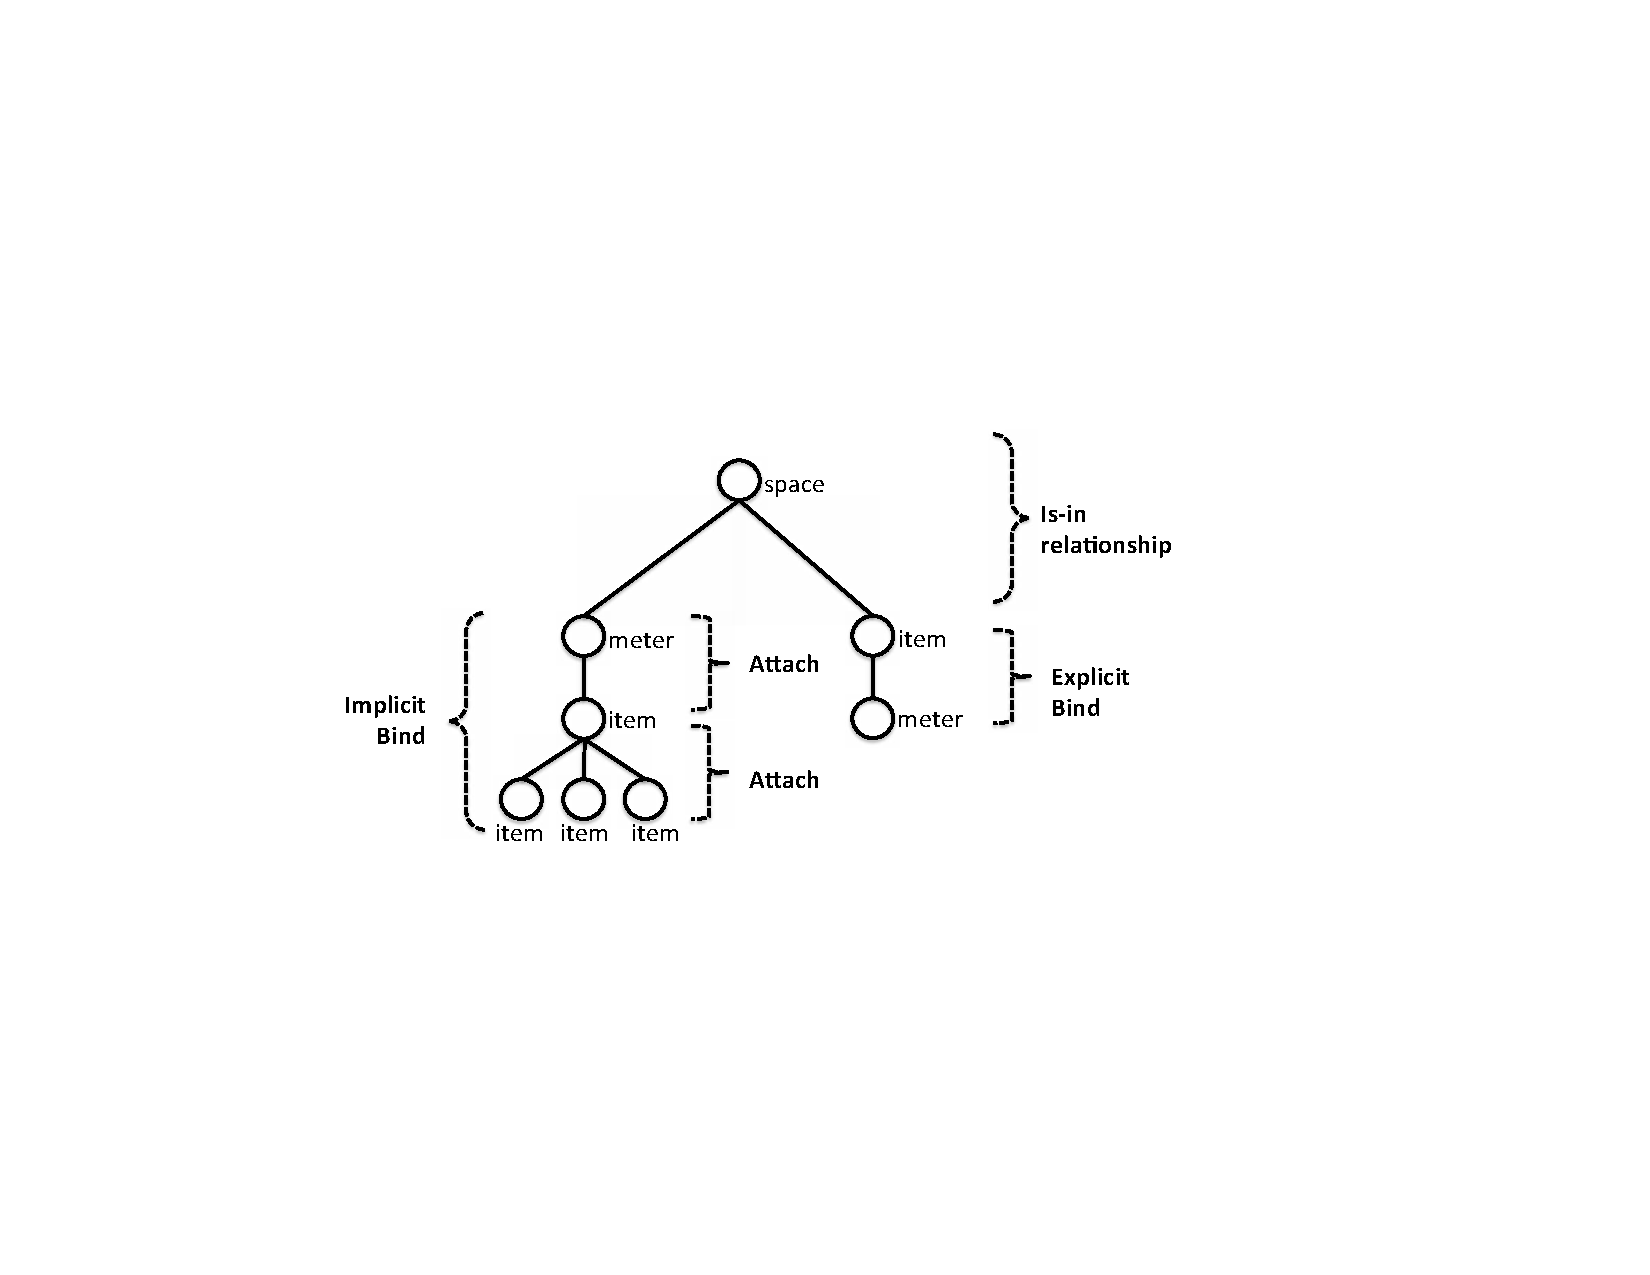
\includegraphics[scale=0.55]{figs/bindattachstructs}
% \caption{This diagram shows the relationship capture between the objects and locations in the building for the 
% energy audit application.  Children of a space node have an ``is-in'' relationship with the space.  An item
% with another item as a child have a ``attached'' relationship and meters attached to items are bound to each other.
% Note, this is a \emph{subset} of the relationship diagrams generated across our three applications.}
% \label{fig:attachandbind}
% \end{center}
% \end{figure}







\subsection{Application layer}
The Energy Lens app consists of a web application that displays timeseries data and an Android-based smartphone
app.
%Figure~\ref{fig:mobileapp} shows a few of screen shots from the application.  
The android app is relatively simple; consisting of a menu with 4 main options: Update deployment state, scan to view services,
scan deployment info QR code, and deployment info.
Swipe gestures manipualte a local portion of the entity-relationship graph -- local with respect to a user's current location.
Since each location (room, floor) has a QR code attached to it and items are associated with those locations, we
can identify the location by name ({\tt /buildings/SDH/spaces/4F/toaster}).  Figure~\ref{fig:swipes} goes through the various sets 
of swipes.


\begin{figure*}[htb!]
\begin{center}
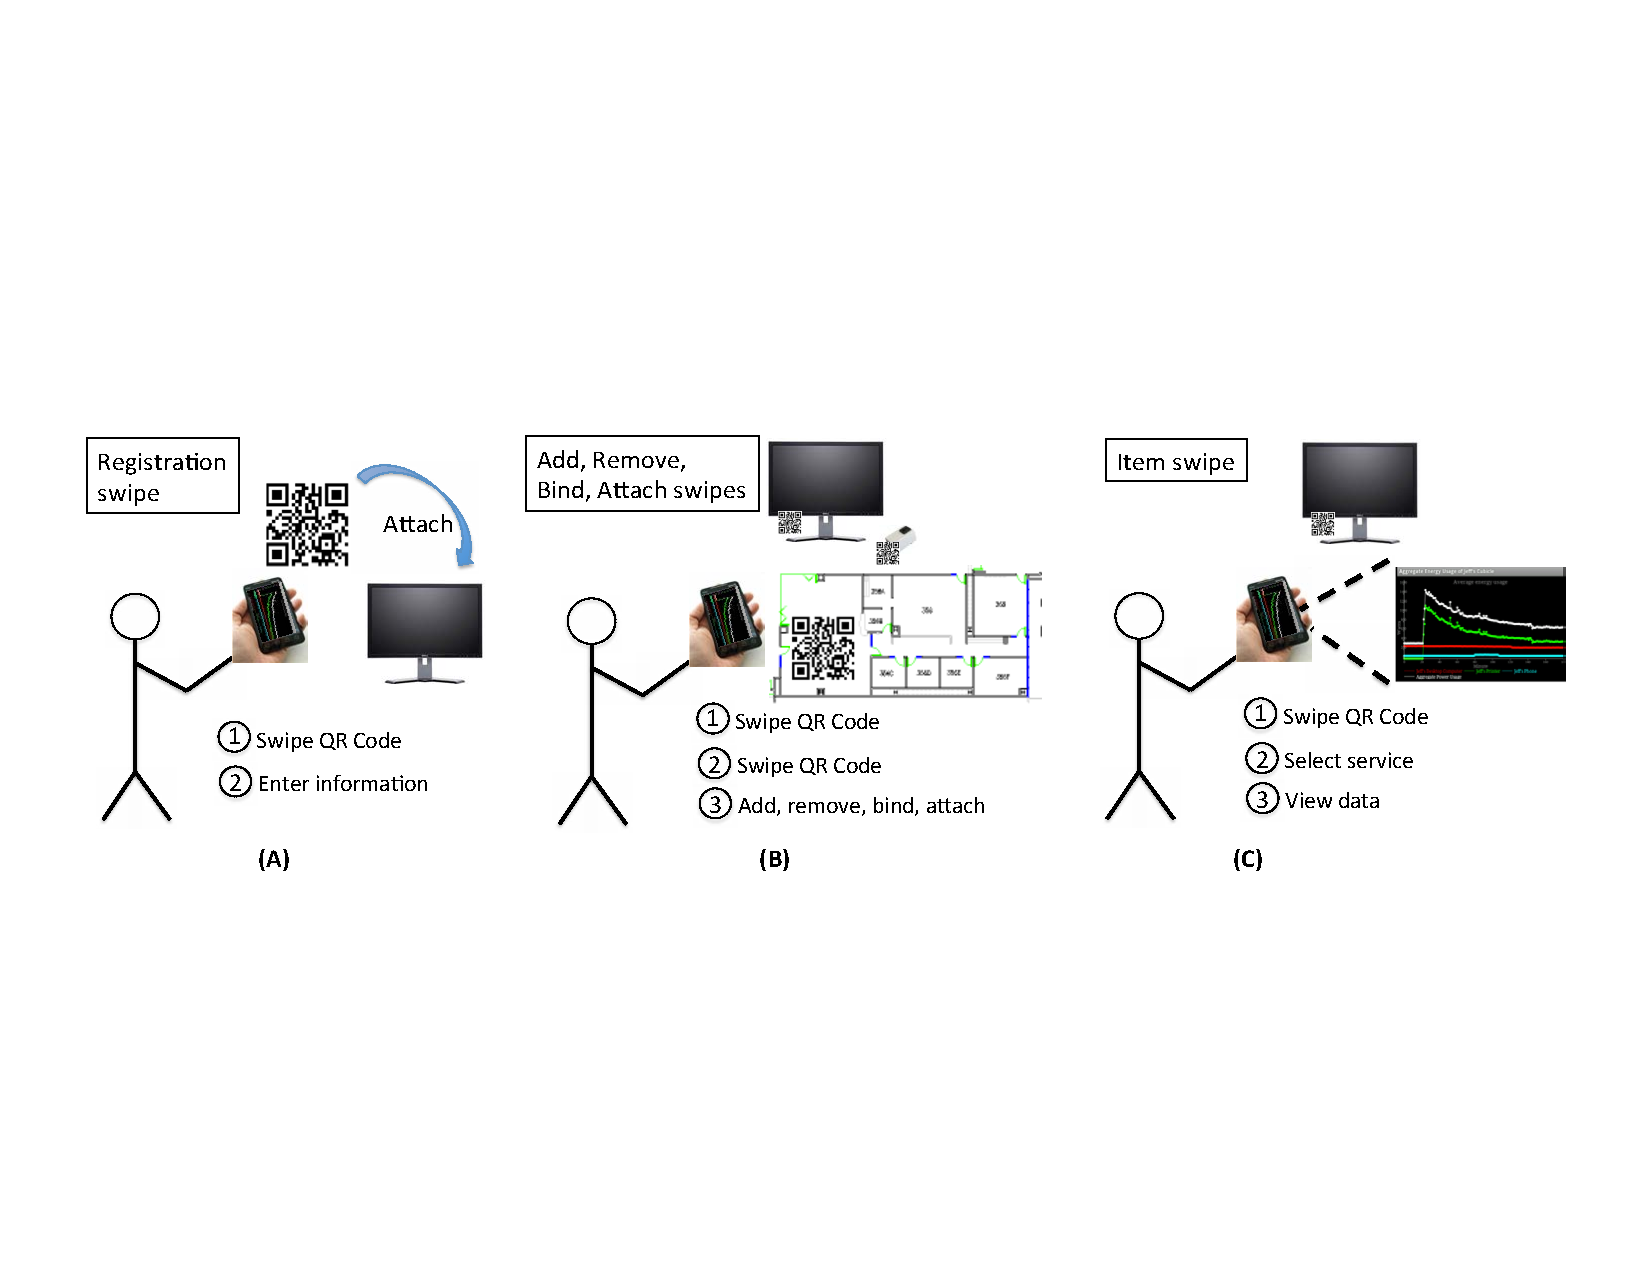
\includegraphics[width=\textwidth]{figs/swipes}
\caption{Swiping gestures in the mobile application that }
\label{fig:swipes}
\end{center}
\end{figure*}

The first set is called a `registration' swipe and we use it to register new items.  The user scans QR code and the item it's attached
to.  This creates an `attached-to' link between them.  Adding, removing, binding, and attaching items is done with a pair of swipes.
A lookup is done with by swiping the QR code attached to an item.


\begin{figure}[htb!]
\begin{center}
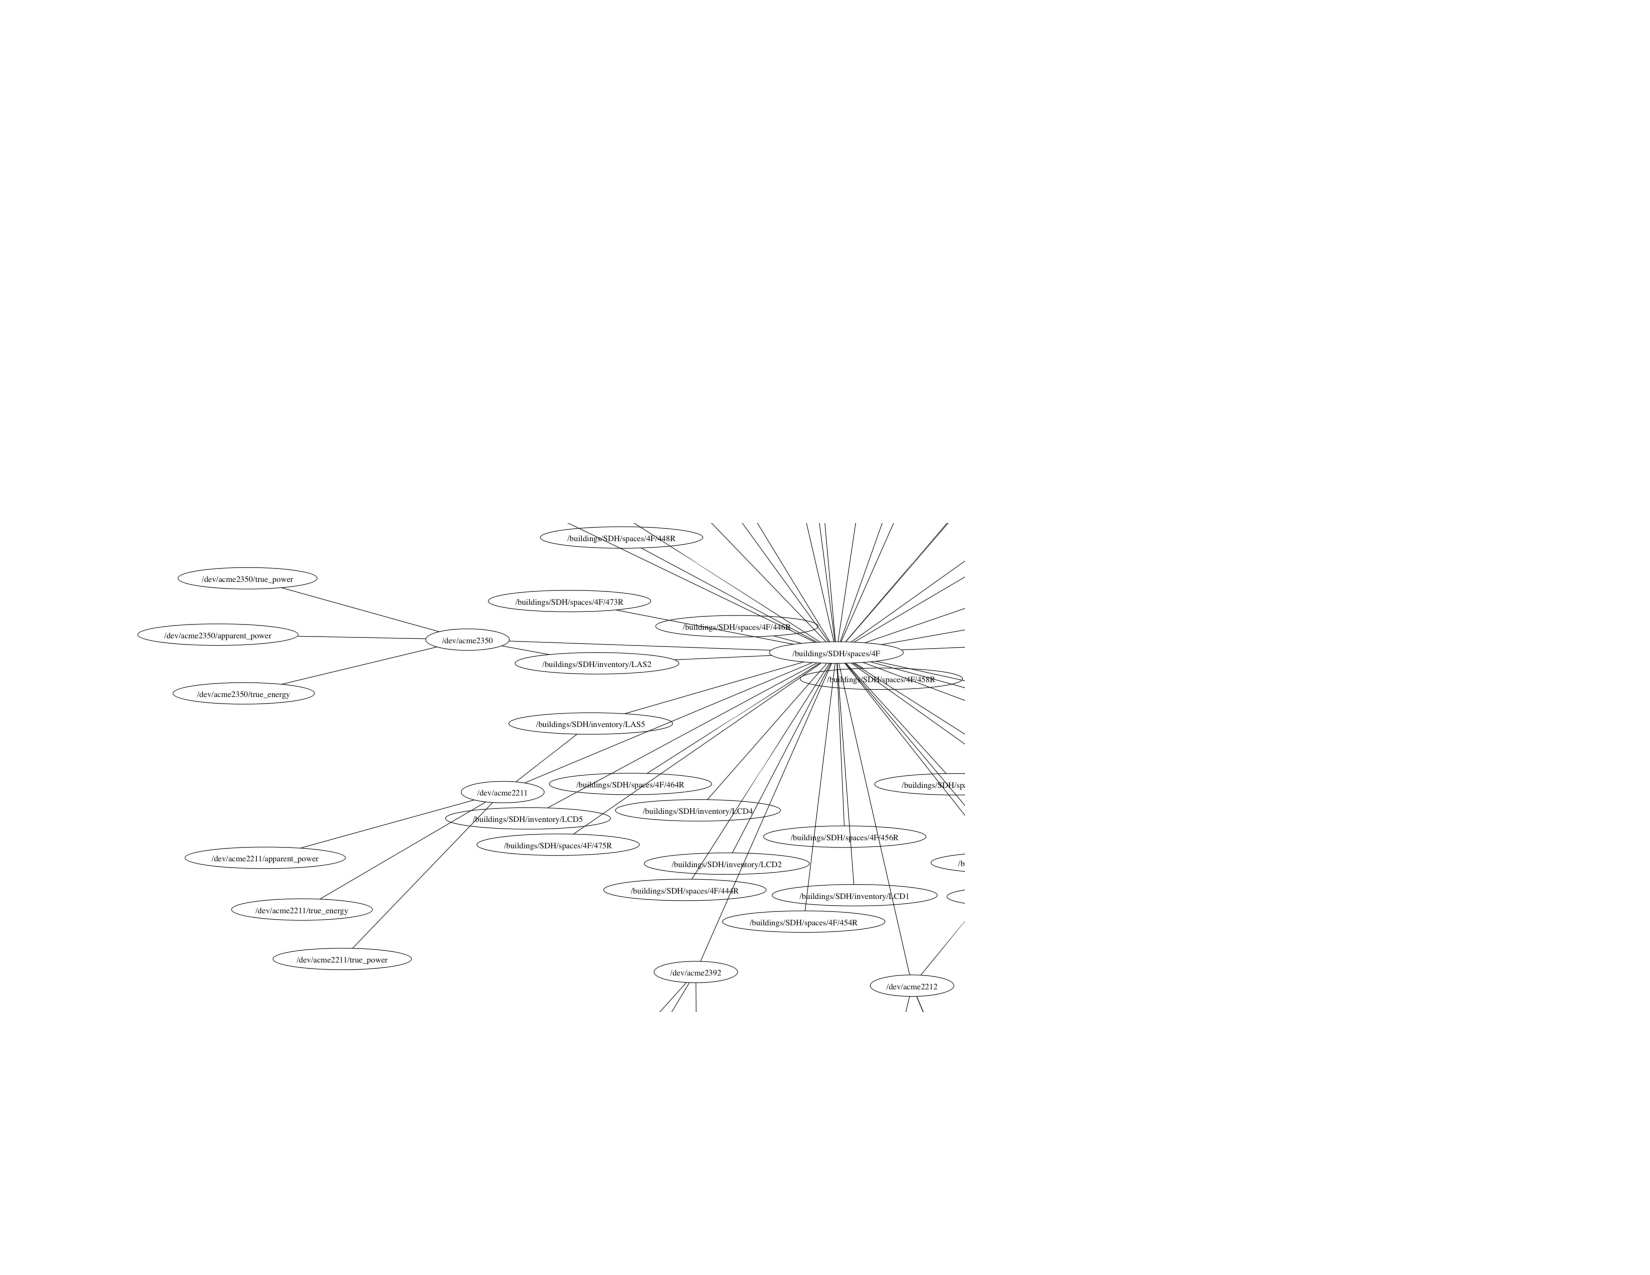
\includegraphics[scale=0.45]{figs/SDH_4F_ERG_closeup}
\caption{A portion of the prefetched entities on the a single floor in our building.  This shows a snapshot of the entity-relationship
graph for that floor.  Each node, link, and associated content is prefetched when the user swipes the floor
tag or anything on that floor.}
\label{fig:sdh_4f_erg}
\end{center}
\end{figure}

\subsubsection{Tracking people and things}
\label{sec:tracking}
% There are three major components in our architecture: QR codes, mobile phones, and StreamFS.

% How do we evaluate our ability to track people and things?
% This is a description evaluation.  We need to describe how the pieces interact.  What will fall out of the description is our strong dependence on occupants/users to give us information about the state of the physical world.  It’ll also fall out that what allows these pieces to fit together is network infrastructure.
We have designed a set of heuristics for setting the location during an update, that piggybacks on the swipe gesture.
The following is a list of rules for automatically setting the location of people and things:

\begin{itemize}
\item When a user swipes a location L, they are presumed to be at L for fixed period $\tau$.  An association timer is set to 
		release this association after $\tau$ seconds.
\item If the user swipes anything that is associated with a location $l$ at time $t \le \tau$, and $l(t)\ne$ L, 
		then we set the new location of \emph{thing} they swiped to l(t) and reset the association timer.
\item If the user swipes anything at location l at time $t \ge \tau$, we set the location of the \emph{person} to l(t).
		We set the association timer to $\tau$.
\item If a user registers a new location, they are presumed to be at that location.
\end{itemize}
\vspace{0.08in}


For each of these, we provide an interactive option to ask for location-change confirmation from the user.  So if we think the
user/item has moved but they have not, the preset action can be overriden.  The guiding principal we follow in our design
is to leverage the swipe gesture for as much contextual information as possible.  Furthermore, we do not explicitly track users.
Context is set on the phone and it represented as the root node in the ERG.
%  which you are either editing directly or
% adding creating/destroying a relationship link in the graph.

Because location swipes give us direct confirmation of a user's location, it can be coupled with wifi localization mechanisms
and supervised learning algorithms to adjust the localization model as the user interacts with their environment. 
For future work we intend to experiment with this mechanism.% to enable supervised-learning-based indoor wifi localization.


\subsubsection{Disconnected operation}
Although connectivity is ubiquitous, network access is not.  There are various reasons for this, including dead zones, 
idle-disconnect and failed hand-off between access points.  When encountered in practice, particularly while editing
deployment state, it can be quite frustrating and discourage use of the application.  We designed a
mechanism that does smart caching, not only to improve performance, but also to allow for disconnected operation.

The Energy Lens application downloads a portion of the ERG when a user enters a new floor.  The application fetches the portion
of the graph rooted at the floor.  
Figure~\ref{fig:sdh_4f_erg} shows just a small portion of that entity-relationship graph for the floor we are monitoring in
our deployment.  A prefetch populates the cache with all entity nodes on that floor, their associated metadata,
and 30 minutes of data from the stream entities.  The full fetch of the 4th floor data set includes
176 nodes and about 1 MB of meter data.  In total, the app downloads ~1.2 MB of data upon re-connection.
Prefetching allows users to continue interactacting with the application as if they were still connected (as long as they remain on
the same floor).  Without it, the application is not functional until a network connection is established.

\begin{algorithm}
\caption{Prefetch Loop}
\label{alg:prefetch}
	\begin{algorithmic}
	\While {true}
	\If {connected and active}
	    \State $req\gets [t_{i-n}, OP_R]$
	    \State $resp\gets $ send($req$)=$[t_{i-k}, OP_R],\dots, [t_{now}, OP_R]; $ 
	    \State $n >= k$
	    \For {$j = 1 \to size(resp)}$
	    	\State $op \gets$ $resp[j]=[t_{i-k+e}, OP_R]$
	    	\State apply($op$)
	    \EndFor
	\EndIf
	\If {active}
		\State Sleep for 10 minutes
	\Else
		\State Sleep for 1 hour
	\EndIf
	\EndWhile
	\end{algorithmic}
\end{algorithm}


Energy Lens periodically syncs with StreamFS to obtain updates to the ERG and maintain a locally consistent view.  
Let $OP_R$ be an operation performed on the node rooted at node $R$ and $t_i$ be the current time on the phone.  
Algorithm~\ref{alg:prefetch} shows the pseudocode for the prefetch process.  After a set period, the phone sends the server
its last performed operation and the time that operation was performed.  The server responds with any operations that have
take place since then.  The client applies those operations internally to the cached version of the the ERG in order to 
maintain consistency.  The ``\emph{active}'' parameter-check, is for energy savings.  If the phone application is active, the
check occurs every 10 minutes, otherwise it occurs ever hour.

The entire process is demonstrated in Figure~\ref{fig:interactions}.  The components shown are the \emph{ERG cache}, the \emph{operation
log (OpLog)}, and the \emph{prefetcher}.  We separate the steps in the figure as a READ sequence and a WRITE sequence.
All reads go to the cache (steps 1 and 2 on the left hand side of the figure).  Writes go through the OpLog (steps 1 - 5 on the right
side of the figure).  For writes, 
the application makes a write request (1) and it is forwarded to StreamFS (2).  If StreamFS is reachable and the write is
successful (3), the operation is applied to the ERG cache (4) and the response is sent the application (5).
If the operation is not successfuly, step 4 is skipped.  If StreamFS could not be reached, step 3 is skipped, and the operation
is written to the OpLog.  The OpLog is flushed to the server, by the prefetcher, upon re-connection.  
% If there are any operations 
% that were applied 
% to the cache that were not applied on the server, they must be applied to the server.

The OpLog contains records of operations that are eventually applied to StreamFS.  Some of those operations
are actually groups of operations that need to be applied atomically.  For example, 
when a bind or attach operation occurs, we append the timestamp to the item(s) that are being connected, as well as create
a link between them in the graph.  The application uses both the link and the added metadata to fetch the appropriate
graph for display.  These operations must be applied atomically or not be applied at all.
When the log is dumped, the global transaction manager (GTXM) -- the layer that handles log dumps and transaction processing --
attempts to apply the log in timestamp order.

% \subsubsection{consistency \& disconnected operations}

% The ability to provide real-time analytics for physical data application is driven by 

% The consistency and accuracy that we capture about the entities in the world and their relationships and associated metadata.
% How those relationships/metadata inform our analytical operations.

% Entities in the physical world can be difficult to capture and track over time.  Ideally we’d have a model of the world and the things in it and there would be a mechanism for tracking things that move.  We approximate this mechanism through the combination of QR codes, mobile phones, and people.  Items in the real-world are physically tagged with a QR code that serves as a reference for the “thing” in the physical world.  The mobile phone gives the person a ubiquitous QR code reader.  It also serves to provide the person with services associated with the physical world.

% \subsubsection{Caching}
% Although network connectivity is theoretically ubiquitous, in practice, this is not always the case.  In order to enable updates while disconnection we need to cache as much of the relevant deployment state as possible.

% \subsubsection{Pre-fetching \& The state-change stream}
% We should pre-fetch, as the tags inform us about what the user might access next.  What are some things to pre-fetch?  All the paths from the current root to the leaves.  We should also fetch the object associated with each file and for streams, we should fetch 1 hours’ worth of data.  In most cases this means fetching about 200-400 KB of data.


\begin{figure}[htb!]
\begin{center}
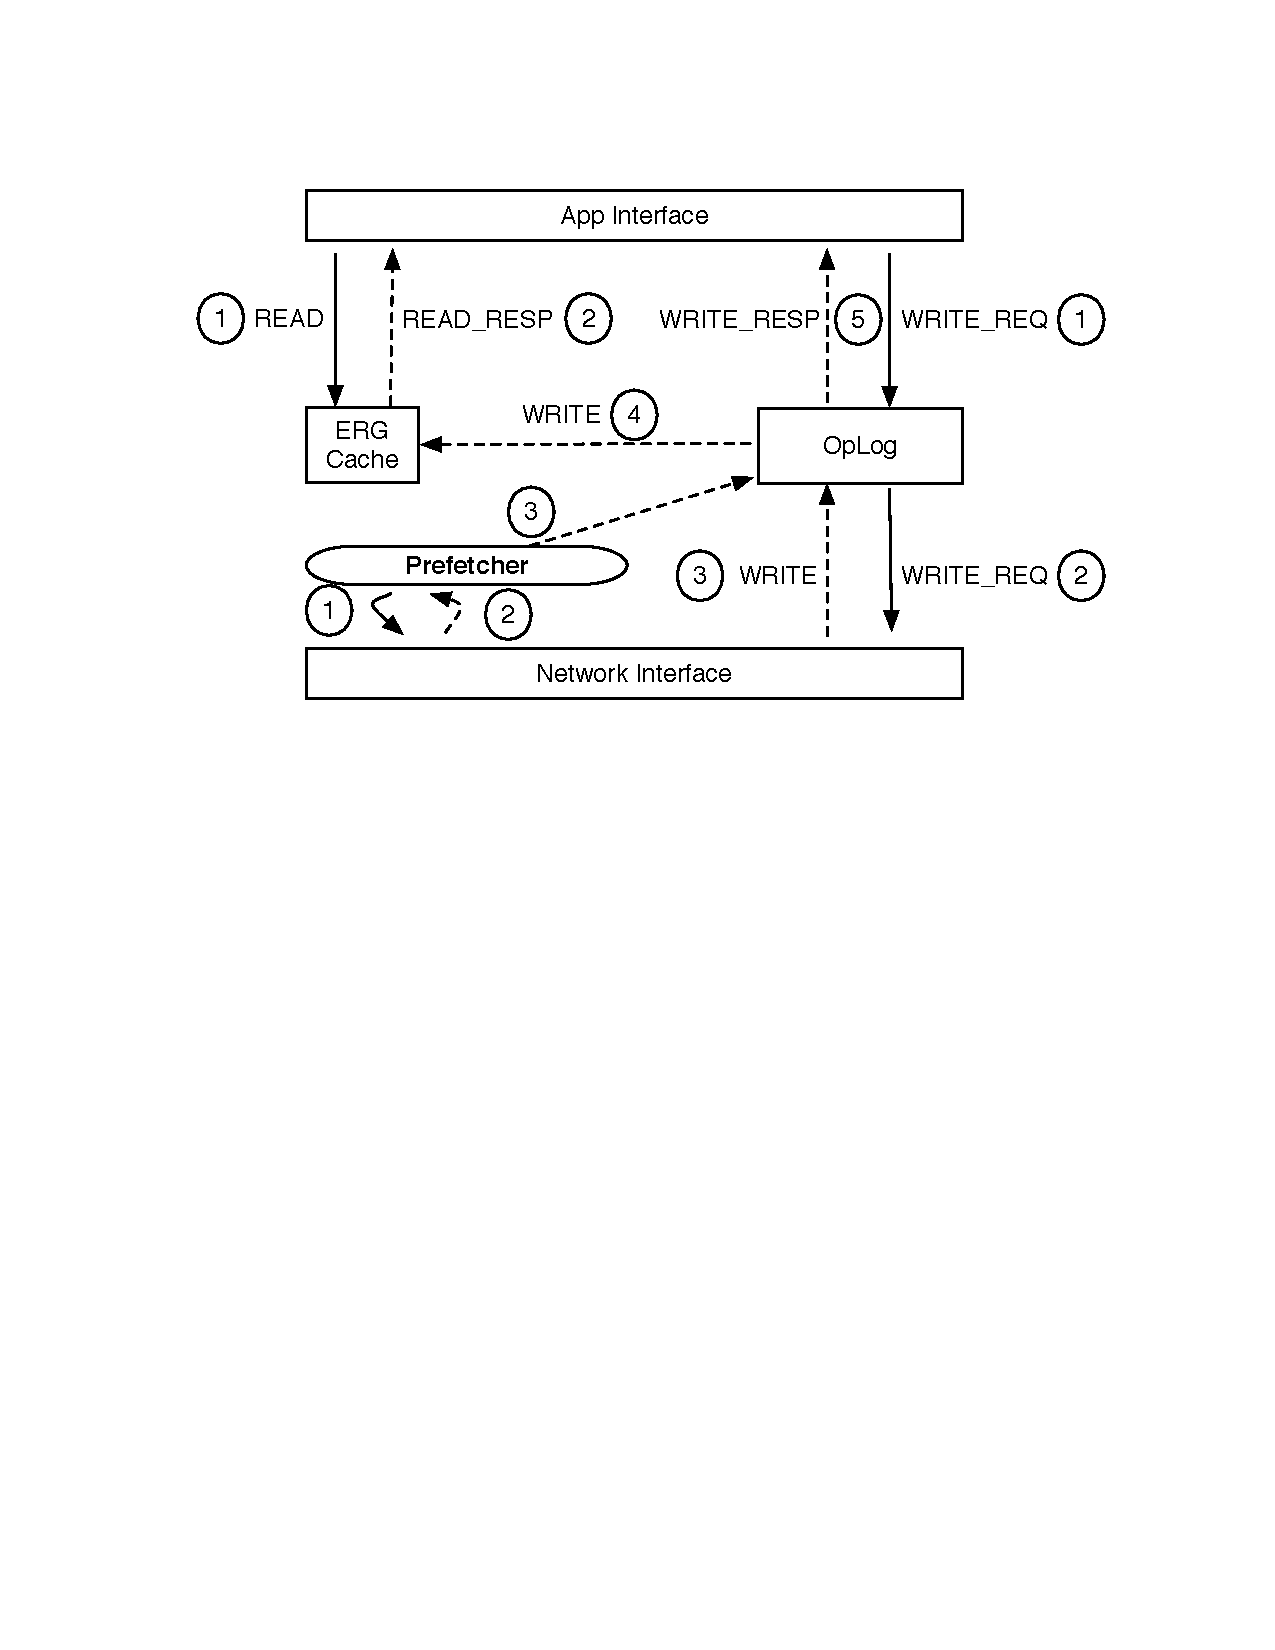
\includegraphics[scale=0.50]{figs/standard_interaction}
\caption{Standard mechanisms for consistency management on the phone.  All READ request go to the local
cached version of the ERG.  All WRITES must go through the OpLog.  They are eventually applied to the cache
if successful and logged if the StreamFS is unreachable.}
\label{fig:interactions}
\end{center}
\end{figure}

\subsubsection{Log dumps and conflict resolution}
\label{sec:conflicts}
When the Energy Lens application is started it makes contact with the server and attains the server's local clock time. 
It notes the local time and as being equal to the timestamp of the server and calculates all subsequent timestamps
using its local clock.  When an operation or transaction is add to the OpLog, a timestamp is appended.  Let $t_s$ be the timestamp 
on the server, $t_l$ be the timestamp on the phone when $t_s$ is recorded, and $t_{now}$ be the current time on the phone.  
Each operation/transaction is timestamped with $t_{approx}$ where:

\begin{equation}
t_{approx} = t_s + (t_{now} - t_l)
\end{equation}


This timestamp is a general approximation of when the operation should be applied on the server.  The server timestamps
to order operations when replaying and applying logs.

Generally, a conflict occurs if there is any operation or transaction that was applied after the timestamp of the current operation
being processed.  A typical transaction manager must rollback the state of the database, apply the operation, and replay
the log.  However, conflict resolution is much simpler in this context.  \emph{The latest operations reflect the state of the
world because they are updates induced by direct interaction with the world at that point in time.}  Therefore, if there is a conflict
between a set of operations, the old ones can all be discarded.
% When this happens the GTXM does a rollback operation.  The rollback operation
% fetches all the oepration that need to be ``undone'', generates the negative operation, and applies them to StreamFS.
% StreamFS has no notion of an operation log and all state is maintained by the GTXM.  After the rollback is finished, 
% an attempt is made to apply the pending operation/transaction.  If it succeeds, the ``undone'' operations are re-applied.
% If it fails, it is placed in a failure log and the undone operations are re-applied.  Every successfully applied operation is logged
% to a success log.
Operations that are discarded are done so silently.  We make failures silent for two reasons: 1) There is no way to contact the app when 
failure occurs.  Mobile phones
do not often have reversably reachable addresses.  2) Failure assumes the operation was based on a false assumption about the state
of the world.  
% However, this does not fully cover all cases.  It may be the case that
% there the state of the world was not reflected in StreamFS or the user's phone and that it was reflected on some else's phone that
% has not done a log dump yet.  We do not currently handle this case, however, we may be able to address it by attempting to re-apply
% failed operations that are logged in the failure log.


% when an operation has a timestamp larger than the


% Once the transaction/OpLog is dumped the server the server attempts to apply it in StreamFS.
% When a transaction with an earlier timestamp than the last committed transaction is offered, the EnergyLens transaction manager checks 
% if the current transaction conflicts with any previously committed transaction.  This is done by checking if the files that are touched 
% overlap with a transaction that touches the same files and has a transaction timestamp that’s later than the current transaction being offered.  
% If so the transaction manager rolls back the state of StreamFS, only for the affected files, back to the last transaction before the last commit.  
% It then commits the offered transaction, adds it to the transaction log, and replays the transaction that was rolled back.  
% If the operations of the replayed transaction are no longer valid, the transaction fails silently.  Failing silently is acceptable in 
% this context because we want to capture the latest state of the world.  By rejecting the transaction, we are assuming that it was based 
% on false assumptions about the state of the world.  We believe this assumption to be true in most cases.


% \subsubsection{Maintaining, representing, and using physical state and inter-relationships}
% In order to provide relevant services, we need to capture the state of the physical environment within the building.  By “relevant”, we mean based on context and inter-relationships.  What are “the relevant services” we’re talking about?

% \begin{itemize}
% \item Energy analytics on the physical world.
% \item How much does this floor consume?
% \item What fraction of that is going to the various energy-related categories?  plug-load, hvac, lighting.
% \item Personalized energy analytics.
% \item Access the the control interface for the physical world.
% \end{itemize}

% \subsubsection{General approach}
% Our approach is to abstractly represents things in the environment as logical entities and to capture their inter-relationships through an entity-relationship graph.  We use the entity relationships to track where objects and things are in the environment, which helps us maintain a more consistent view of the world.  We also use  it to inform our analytical approach and our choice of services to display.

% \subsubsection{Consistency management}
% Connecting the various components requires ubiquitous connectivity.  Although connectivity is available through the building and the access-point deployment is engineered to minimize dead spots, disconnections still occur (timeout, dead-spots, unsuccessful handoffs).  So, we need to design the system to deal disconnect operation.

% Evaluation will be of a protocol description and design rationale described in detail here.
% What’s the evaluation exactly?

% \begin{enumerate}
% \item Time to download the associated contextual information from StreamFS: files, metadata information, data**
% \item Conflict resolution examples**
% \item Optimizations: Pre-fetching measurements**
% \end{enumerate}


\subsection{Real-time analytics}
% Discussion.  What to measure here?  Perhaps we discuss the relevant real-time analytics we run?  Will there be space?  For buildsys, include a half page talking about some of the analytics.

Figure~\ref{fig:tsdata} shows three screen shots of power traces obtained from the ACme deployment.  Notice that there is
some data missing in the graph.  This occurs due to loss in the network due to interference, reboots on the data management layer,
or failed scripts that are automatically restarted.  In all cases we get holes in the data and to compute the aggregate
curve, interpolation is necessary.  StreamFS offers a real-time processing facility, whereby javascript operaters can be applied
on the stream data to clean it as it comes in, and later compute the aggregate trace.  Currently, we have no made use of this facility.

\begin{figure}[htb!]
\begin{center}
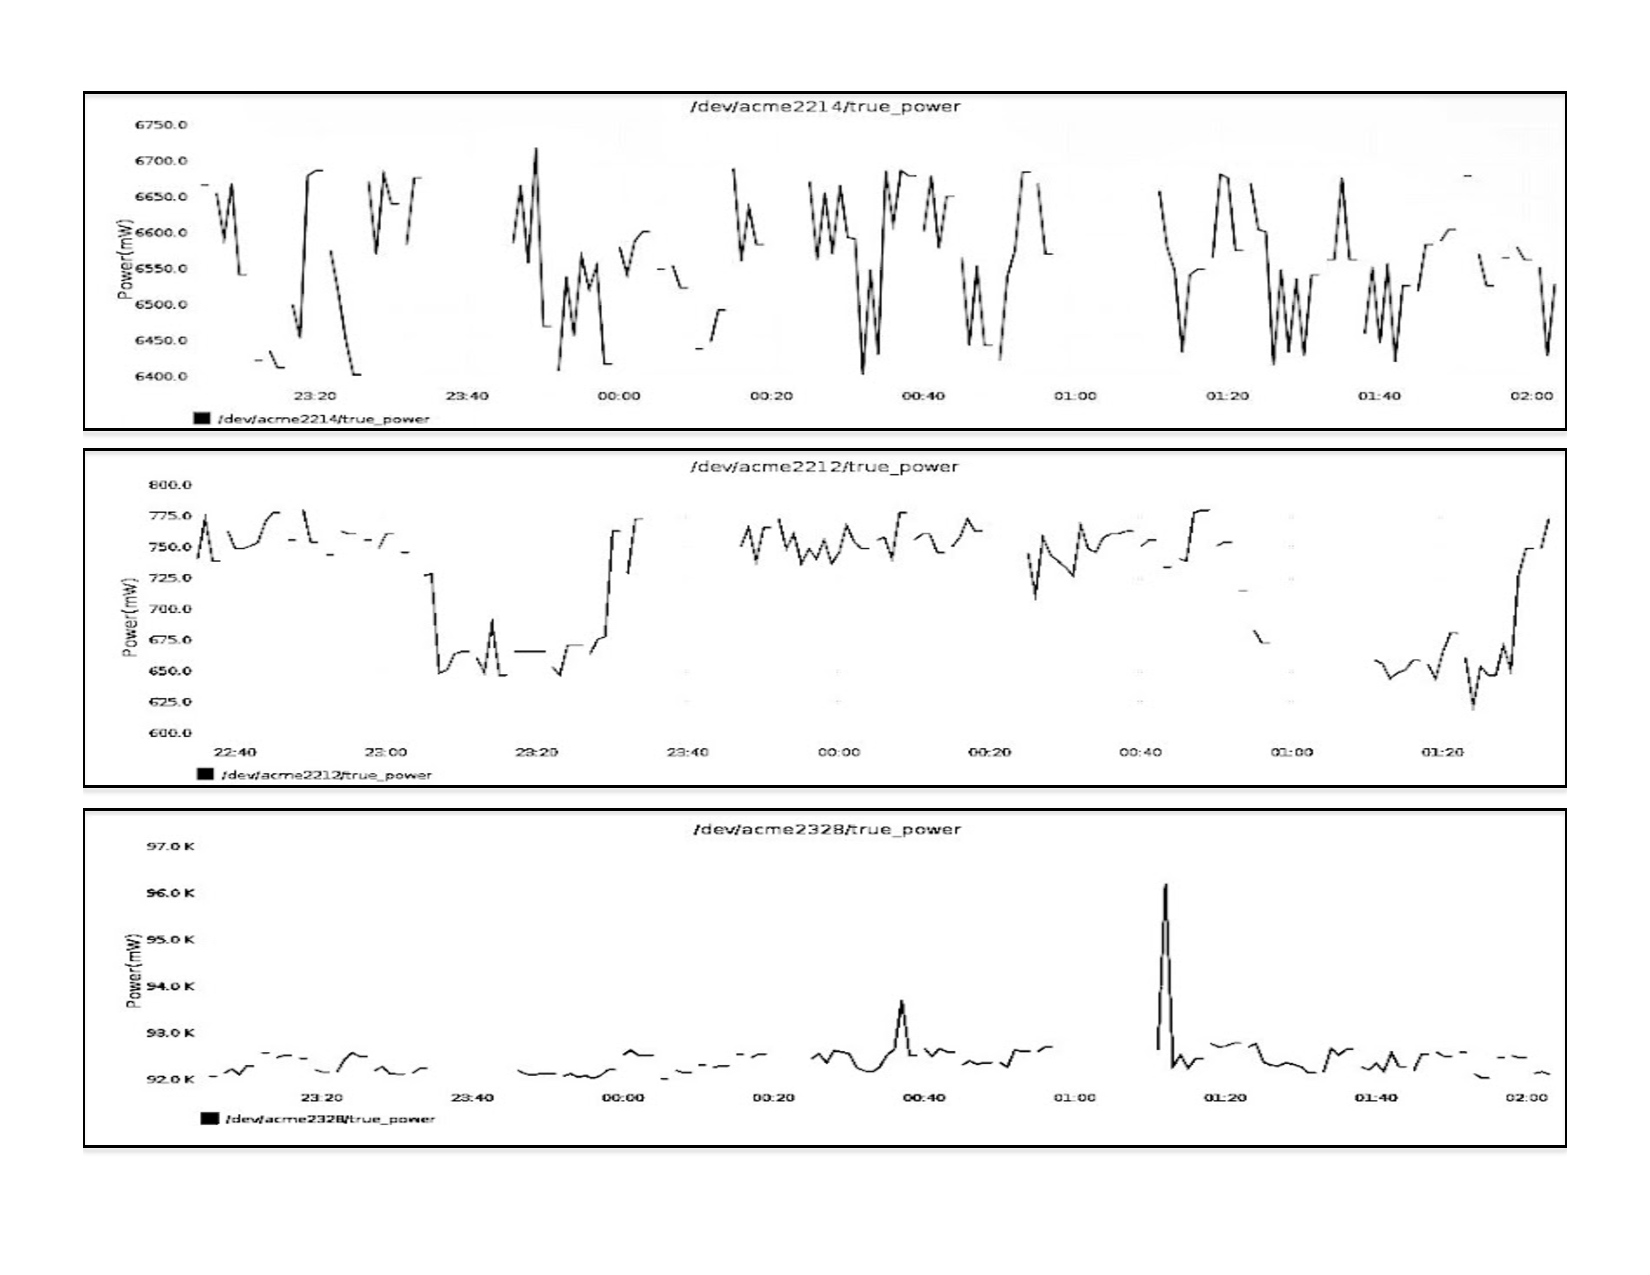
\includegraphics[scale=0.33]{figs/graphs_screen}
\caption{Power traces obtained from power meters attached to various plug load on one of the floors of
a building on campus.}
\label{fig:tsdata}
\end{center}
\end{figure}

However, data modeling is very important in this context.  We wish to use various physical models to clean this dirty data and
other data sources and we increase the number of systems we integrate together.





% Pub/sub architecture
% time decoupling
% variable time-decoupling achieved through the datastore as a buffer
% synchronization decoupling
% Either the publisher or subscriber run asynchronously.
% space decoupling
% The subscriber doesn’t have an explicit reference to the publisher.
% Programming model for real-time data
% Naming/tagging streams
% Dealing with dynamism through tagging
% Built-in functions for physical data
% heat modeling
% electrical modeling
% mathematical modeling

% Security and privacy
% Discussion.  Various topics related to StreamFS here.  Also some topics related to managing security in StreamFS for doing control.  Include another half page, perhaps.


% * Experiment that we need to run.\\
% ** Code that needs to be written and experiment that needs to be run